\section{原子 原子量}\label{sec:1-5}

\subsection{原子}

分子是很小的,它是否可以再分呢?

实验证明,物质的分子能够经过化学反应而变成其它物质的分子,可见,分子尽管很小,但还是可分的。
例如,氧化汞受热时,氧化汞分子分解为更小的氧和汞的微粒,这些更小的微粒经过重新组合,成为氧分子和金属汞。
科学上把这种用化学方法不能再分的微粒叫做原子。用化学方法不能把氧或汞的微粒进一步分成更小的微粒,
这种氧的微粒就是氧原子,汞的微粒就是汞原子。

每个氧化汞分子是由一个氧原子和一个汞原子构成的。
在氧化汞的分解反应里,每个氧化汞分子分解成一个氧原子和一个汞原子。
氧原子和汞原子各自重新组合成氧分子和金属汞。
这个反应可以用图式形象地表示如下:

\begin{figure}[htbp]
    \centering
    \begin{tikzpicture}[
    myarrow/.style={line width=3pt, -{Stealth[length=5mm]}, gray},
]
    \tikzset{
        oxygen/.pic={% 绘制 “氧原子”
            \shade[ball color=gray!20] (0, 0) circle (.5cm);
            \draw[pattern={mylines[angle=0, distance={3pt}]}] (0, 0) circle(.5cm);
        }
    }

    \begin{scope}[yshift=2cm]
        \shade[ball color=black!50] (0, 0) circle (.6cm);
        \draw (1.1, 0) pic {oxygen}
            node[below=0.6cm, xshift=-0.5cm] {氧化汞分子};

        \draw [myarrow] (3, 0) -- (4, 0);

        \shade[ball color=black!50] (5, 0) circle (.6cm) node [below=0.6cm] {汞原子};
        \node at (5.8, 0) {\Large $+$};
        \draw (6.6, 0) pic {oxygen} node[below=0.6cm] {氧原子};
    \end{scope}

    \begin{scope}
        \draw (0, 0) pic {oxygen} node[below=0.6cm] {氧原子};
        \node at (0.8, 0) {\Large $+$};
        \draw (1.6, 0) pic {oxygen} node[below=0.6cm] {氧原子};

        \draw [myarrow] (3, 0) -- (4, 0);

        \draw (5, 0) pic {oxygen}
              (6, 0) pic {oxygen}
              node[below=0.6cm, xshift=-0.5cm] {氧分子};
    \end{scope}
\end{tikzpicture}


\end{figure}


从上述分析还可以说明原子和分子的不同。在化学反应里,分子可以分成原子,而原子却不能再分。
构成氧化汞分子的氧原子和汞原子在化学反应后,仍然是氧原子和汞原子,并没有变成其它原子,因此,
\zhongdian{原子是化学变化中的最小微粒。}

人们通过实验和论证,知道了原子的存在。用现代科学仪器能拍摄出反映钨原子的照片(图 \ref{fig:1-11}),
图中每一个小亮点代表一个钨原子。本书封面底纹,也是显现原子图象的一张照片。

\begin{figure}[htbp]
    \centering
    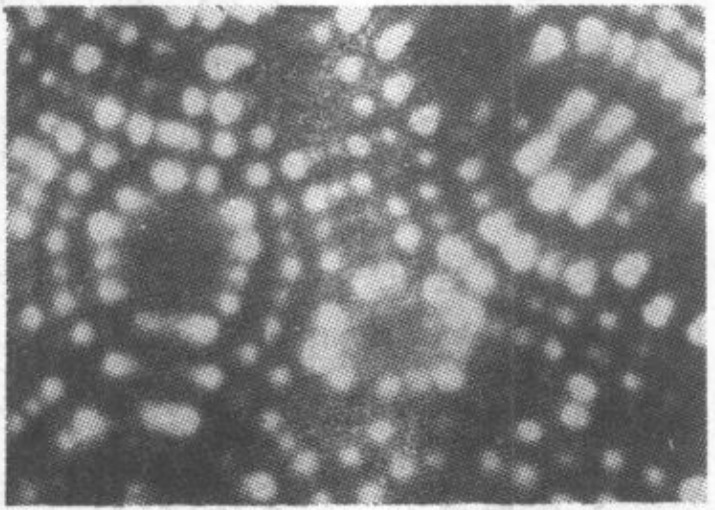
\includegraphics[width=9cm]{../pic/czhx1-ch1-11}
    \caption{用现代科学仪器拍摄的金属钨的照片(放大 $200$ 万倍)}\label{fig:1-11}
\end{figure}

原子和分子一样,也是在不断地运动着的。

原子很小,我们如果有可能把一亿个氧原子排成一行,它们的长度也不过只有一厘米多一些。

有些物质是由分子构成的,还有一些物质是由原子直接构成的。
例如,钨是由许多钨原子构成的,汞是由许多汞原子构成的,铁是由许多铁原子构成的。

人类对物质结构的认识可以追溯到古代。
远在公元前五世纪,希腊哲学家德谟克利特\footnote{德谟克利特(Democritus, 公元前 460? —\, 370?)。}等
人认为万物是由大量的不可分割的微粒构成的,并把这些微粒叫做原子(希腊文原意是“不可分割”)。
这种古代的原子观念是人们根据对自然界的观察,想象和推测提出来的,没有经过实践的验证。
到了十九世纪前半世纪,随着科学技术的发展,积累了大量事实,论证了原子和分子的存在。
在这期间,英国科学家道尔顿\footnote{道尔顿(Dalton, 1766 —\, 1844)。}提出了近代原子学说,
他认为物质是由原子构成的,这些原子是微小的不可分割的实心球体,同种原子的性质和质量都相同,等等。
道尔顿的近代原子学说对化学的发展起了十分重要的作用。但他没有把原子和分子区别开来。
后来,意大利科学家阿佛加德罗\footnote{阿佛加德罗(Avogadro, 1776 —\, 1856)。}提出了分子的概念,
指出了分子和原子的区别和联系。人们把物质由原子、分子构成的学说叫做原子-分子论。

自从用原子-分子论来研究化学反应后,化学才开始成为一门科学。
现在,人们对物质结构的认识早已远远地超过了原子-分子论的水平。
由于科学技术的迅速发展,我们对原子、分子的认识已越来越深入。



\subsection{原子是由什么微粒构成的呢?}

原子是不是最小的微粒,能不能再分呢?

直到十九世纪末,人们还认为原子是不能再分的。后来,生产技术的发展为精密的科学实验提供了条件。
1897 年,在英国科学家汤姆生\footnote{汤姆生(Thomson, 1856 —\, 1940)。} 发现电子以后,
人们开始揭示了原子内部的秘密,认识到原子不是最小的微粒,而是具有复杂的结构,还可以再分。

现代科学实验已经证明,\zhongdian{原子是由居于原子中心的带正电的原子核和核外带负电的电子构成的。}
由于原子核所带电量和核外电子的电量相等,但电性相反,因此原子不显电性。
不同类的原子,它们的原子核所带的电荷数彼此不同。如
氢原子,原子核带 $1$ 个单位正电荷,核外有 $1$ 个电子,即 $1$ 个单位负电荷;
氧原子,原子核带 $8$ 个单位正电荷,核外有 $8$ 个电子,即 $8$ 个单位负电荷等等。
原子核比原子小得多,原子核的半径约为原子半径的万分之一,原子核的体积只占原子体积的几千亿分之一。
假设原子有一座十层大楼那样大,那么原子核却只有一个樱桃那样大。
因此,相对来说,原子里有一个很大的空间。电子在这个空间里作高速的运动。

原子核虽小,但还可以再分。现代原子能的利用、原子弹的爆炸,就是利用了原子核裂变时所放出的巨大的能量。

科学实验证明,\zhongdian{原子核是由质子和中子两种微粒构成的。}
每个质子带 $1$ 个单位的正电荷,中子不带电,可见原子核所带的正电荷数(即核电荷数)就是核内质子的数目。
表 \ref{tab:1-1} 列了几种原子的构成。

\begin{table}[htbp]
    \centering
    \caption{几种原子的构成}\label{tab:1-1}
    \begin{tblr}{
        hline{1,12}={1.5pt,solid},
        hline{2,3}={solid},
        vlines,
        vline{1,5}={1.5pt,solid},
        %columns={c},
        colspec={
            cQ[si={table-format=2},c]
            Q[si={table-format=2},c]
            Q[si={table-format=2},c]
        },
        row{1,2}={guard},
    }
        \SetCell[r=2]{m} 原子种类 & \SetCell[c=2]{c} 原子核  & & \SetCell[r=2]{m} 核外电子数 \\
        & 质子数 & 中子数 &  \\
        氢 & 1  &    & 1 \\
        氦 & 2  & 2  & 2 \\
        碳 & 6  & 6  & 6 \\
        氧 & 8  & 8  & 8 \\
        氖 & 10 & 10 & 10 \\
        钠 & 11 & 12 & 11 \\
        硫 & 16 & 16 & 16 \\
        氯 & 17 & 18 & 17 \\
        铁 & 26 & 30 & 26 \\
    \end{tblr}
\end{table}

原子的结构是很复杂的。人类对原子结构的认识,将随着科学的发展而深化。



\subsection{原子量}

原子虽然很小,但有一定的质量。原子的质量是原子的一种重要性质。原子的质量各不相同, 例如:

一个碳原子的质量是:$0.000 \; 000 \; 000 \; 000 \; 000 \; 000 \; 000 \; 000 \; 019 \; 93$ 千克,
即 $1.993 \times 10^{-26}$ 千克。

一个氧原子的质量是:$0.000 \; 000 \; 000 \; 000 \; 000 \; 000 \; 000 \; 000 \; 026 \; 57$ 千克,
即 $2.657 \times 10^{-26}$ 千克。

一个铁原子的质量是:$0.000 \; 000 \; 000 \; 000 \; 000 \; 000 \; 000 \; 000 \; 092 \; 88$ 千克,
即 $9.288 \times 10^{-26}$ 千克。

这样小的数字,书写、记忆和使用都很不方便,就象用吨来表示一粒稻谷或小麦的质量一样。
因此,在科学上,一般不直接用原子的实际质量,而采用不同原子的相对质量。
国际上是\zhongdian{以一种碳原子\footnote{这种碳原子指的是原子核内有 $6$ 个质子和 $6$ 个中子的一种碳原子。此外,还有质子数相同而中子数不同的碳原子。}的
质量的 $1/12$ 作为标准,其它原子的质量跟它相比较所得的数值,就是该种原子的原子量。}
例如,采用这个标准,测得最轻的氢原子量约等于 $1$,氧原子量约等于 $16$,铁原子量约等于 $56$ 等等。
由此可见,原子量只是一个比值,它是没有单位的。我们采用原子量来计算、书写和记忆就都很方便了。
一般化学计算是采用原子量的近似值,见第 \pageref{tab:1-2} 页的表 \ref{tab:1-2}。
国际原子量表见书末附录 I。

原子是由质子、中子和电子构成的。根据实验测定,
质子的质量等于 $1.6726 \times 10^{-27}$ 千克,
中子的质量等于 $1.6748 \times 10^{-27}$ 千克,质子和中子的质量约相等,都约等于一种
碳原子\footnote{这种碳原子指的也是原子核内有 $6$ 个质子和 $6$ 个中子的一种碳原子。}质量的 $1/12$,
即约等于一个氢原子的质量。它们都约是电子的质量的 $1836$ 倍。
电子的质量很小,原子的质量主要集中在原子核上。


\begin{xiti}

\xiaoti{用分子、原子的观点解释下面两种变化在本质上有什么不同:酒精的挥发;磷燃烧生成五氧化二磷。}

\xiaoti{有人说,物质都是由分子构成的,对不对?试举例说明。}

\xiaoti{选择正确的答案填写在括号里。}
\begin{xiaoxiaotis}

    \xxt{原子核 \ewkh 。\\
        \tc{1}由电子和质子构成, \tc{2}由质子和中子构成, \tc{3}由电子和中子构成,\tc{4}不能再分。
    }

    \xxt{在原子里质子数等于 \ewkh 。\\
        \tc{1}中子数, \tc{2}电子数, \tc{3}中子数和电子数之和。
    }

    \xxt{碳的原子量是 \ewkh 。\\
        \tc{1}12 克, \tc{2}12, \tc{3}$1.993 \times 10^{-26}$ 千克。
    }

\end{xiaoxiaotis}


\xiaoti{以氧原子为例,说明构成原子的微粒有哪几种。它们怎样构成原子?为什么整个原子不显电性?}

\xiaoti{查阅书末附录 \ref{app:1} \nameref{app:1},把原子量填在下列空格里。\\
    \begin{tblr}{hlines, vlines, colsep=2em}
        名称   & 氢 & 氧 & 钠  & 氯 & 碳 & 铁 \\
        原子量 &    &    &     &    &    &
    \end{tblr}
}

\end{xiti}


